\section{2D eigenstates}
\subsection{Dummy}

\begin{frame}{Groundstate of the \AB\ tiling}
\(
\<{8cm}
\centering
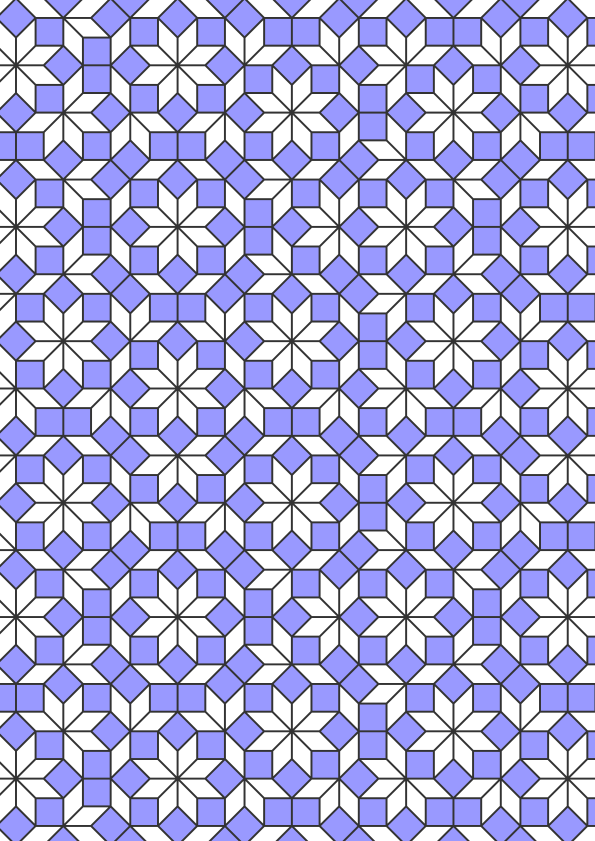
\includegraphics[width=.8\textwidth]{img/4_part3/ammann}

{\ss A patch of the \AB\ tiling}
\>
\<{7cm}
Hamiltonian:
\[
	\op{H} = -t\sum_{\langle m,n\rangle} \ket{m}\bra{n} + \sum_m V_m \ket{m}\bra{m}
\]
Quasiperiodicity encoded in adjacency and on-site potentials
\>
\)

\textbf{Fractal} states described by \textbf{height} functions?
\[
	\psi(m) = C(m) e^{\kappa h(m)}
\]
\end{frame}

\begin{frame}{Looking for arrows}
\(
\<{7cm}
Like Fibonacci, \AB\ has a substitution rule:

{\centering
\includegraphics[width=.8\textwidth]{img/4_part3/AB_inflation}
}

$\to$ scale invariance.

Height requires a field of arrows:
\begin{itemize}
	\item irrotational
	\item invariant under substitution
\end{itemize}
\>
\<{7cm}
\AB\ $\to$ notched tiles\dots

{\centering
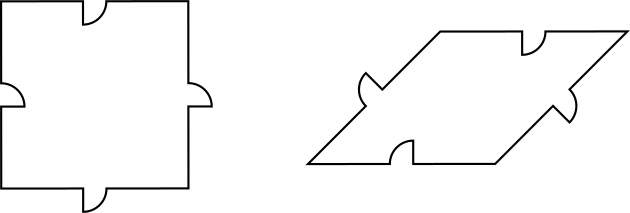
\includegraphics[width=.7\textwidth]{img/4_part3/tiles_notches}

}

\dots exactly what we need!

{\centering
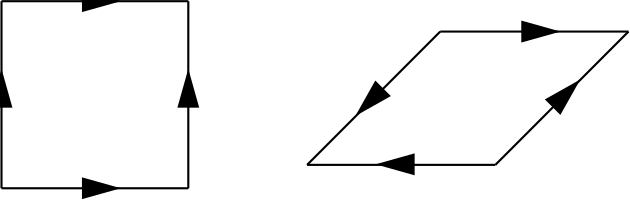
\includegraphics[width=.7\textwidth]{img/4_part3/tiles_arrows}

}

Height field:
\[
	h(m) = \sum_{0 \to m} \text{arrows}
\]
\>
\)
\end{frame}

\begin{frame}{Properties of the height field}

\(
\<{6cm}

{\centering
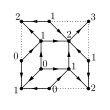
\includegraphics[width=.6\textwidth]{img/4_part3/heights_small_patch}

{\ss The height field on a small patch of the tiling.}

}

\>
\<{8cm}
{\centering
\includegraphics[width=1.\textwidth]{img/4_part3/height_combined}

{\ss Height along a line, shown in blue on the tiling.}

}

Height grows slowly: $h_\text{typ}(L) \simop{L\to \infty} \sqrt{\log L}$

$\to$ states $\psi(m) = e^{\kappa h(m)}$ fractal

\>
\)
\end{frame}

\begin{frame}{Groundstate}

\end{frame}